\chapter{Introduction to gesture recognition}

\section{Classification of gestures proposed in literature}
The vast multiplicity of gestures that human can operate makes the number of classes to which we can divide these gestures is substantial. Therefore the classification can be performed in different ways, taking into account the different characteristics of gestures. Most of presented theories are based on concepts from anthropology, linguistics, cognitive science and others, therefore that include the knowledge which originates from a variety of science. In this chapter it was provided review of the most common gesture classifications in Human Computer Interaction context. It was focused mainly on gestures that are relate to hand and arm movements.

The basic classification of gestures is the division into static and dynamic gestures. Group of static gesture includes fixed gestures which are not taken into account the changes in time, and dynamic gestures is group of time varying gestures.

There is also another general division of gestures considered by Kammer et al. \cite{kammer_taxonomy_2010} due to the type of actions activated by the gesture. It is a division of online and offline gestures. The first one concerns gestures that are processed during gesture performing. It is a group of direct manipulation gestures that provide additional information about dynamics of gesture. There are often used to manipulate objects in space. The second are group of action gestures. They are processed after end of gesture. Most often these are gestures that convey the occurrence of specific meaning.

Karam and schraefel \cite{Karam05ataxonomy} proposed more extensive gesture taxonomy dedicated for Human Computer Interaction. Their classification is based on Quek et al. \cite{Quek:2002:MHD:568513.568514} publication, which provides clarification of gestures taxonomies presented in the past literature. Karam et al. defined following gesture classes: deictic, gesticulation, manipulation, semaphores and sign language. In another publication, Aigner et al. \cite{AignerTaxonomy} presented classification, which are more tailored for hand gesture recognition purposes, drawing on concepts from Karam and schraefel work. They distinguished five categories of gestures:

\begin{figure}[htb]
\centering
 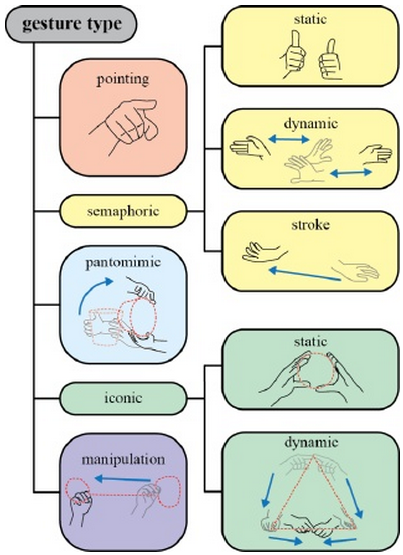
\includegraphics[width=0.5\columnwidth]{figures/gestureTypes.png}
 \caption[]{The classification of gestures proposed by Aigner et al. \cite{AignerTaxonomy}}
 \label{gesturetypes}
\end{figure}

\begin{itemize}
\item pointing -- used to pointing object or indicate direction. Formally, it involve pointing to establish the identity or spatial location of an object within the context of the application domain \cite{Karam05ataxonomy}. It applies not only to indication by the index finger but also to any finger and any number of fingers. It is also independent of finger orientation and curvature, while gesture has a indication meaning. Equivalent of deictic gesture in Karam and schraefel literature.
\item semaphoric -- group which consists of gesture posture and dynamics, which are used to convey specific meanings. Formally, Semaphoric approaches may be referred to as ``communicative'' in that gestures serve as a universe of symbols to be communicated to the machine \cite{Quek:2002:MHD:568513.568514}. Due to the fact that semaphoric are symbolic gesture, their layout can be unrelated to their meaning. Distinguished three semaphoric gesture types of static, dynamic and strokes. The first one concerns specific hand posture, such as thumbs-up meaning approval symbol.
Dynamic semaphorics convey their meaning through movement, for example waving of hand to greet somebody. The last one group are similar to dynamic semaphorics gesture, but this represents fast, stroke-like movements, such as swipe gesture.
\item iconic -- used to demonstrate shape, size, curvature of object or entities. In contrast to semaphoric gestures, their layout or motion path is strictly related to their meaning. Iconic gestures can be divided on static and dynamic. First one are performed by hand postures, such as rectangle formed by the thumb and index fingers of both hands. Dynamic iconic gestures are often used to map edge line of objects by means of motion paths for example showing a simplified sine function characteristics with finger movements.
\item pantomimic -- presents imitated perform of specific task or activity without use any tools or objects. Pantomimic gesture characterized by a high variability of posture and movements. An example of this gesture type can be weapon reload or movement of a knife slicing bread.
\item manipulation -- used to control the position, rotation and scale of the object or entity in space. Manipulation gestures constitute a direct interaction between the manipulated object and hand or tool that performs gesture. It follows that the movement of the manipulated object must be strictly dependent on the motion gesture.
\end{itemize}

\section{State of the art methods}
In this chapter presented review of the state-of-the-art in human gesture recognition. The problem of gesture recognition can be divided in two main problems: the gesture representation problem and the decision/inference problem. Therefore, review includes discussion about enabling technology, gesture representations and analysis of recognition methods. Additionally introduced general problems related to the recognition of gestures and their common solutions.

\subsection{Enabling Technology}
In this subsection, overviewed the enabling technology for gesture recognition. The main existing gesture recognition approaches related to type of the devices are as follow:
\begin{itemize}
\item Non-vision-based devices -- tracking devices, instrumented gloves, armbands and others.
\item Vision-based devices -- using one or many cameras.
\end{itemize}

\subsubsection{Non-vision-based Technology}

This type of devices uses various technologies to detect motions, such as accelerometers, multi-touch screen, EMG sensors and very other include several detectors. There are few categories of non-vision-based \cite{kaaniche2009human}:
\begin{itemize}
\item Wearable -- these kind of device is in the form of garment, which includes sensors needed to recognize arrangement and motions of examined part of body. Often occur in the form of gloves (CyberGlove®), armband (Myo) or the whole outfit (IGS-190). For instance, CyberGlove® device was used in system developed by Kevin et al. \cite{KevinCyberGloves}, which recognize multi-dimensional gestures using condensation-based trajectory matching algorithm. These devices are often related to biomechanical and inertial technologies. 
\item Biomechanical -- type of device, which use biomechanical techniques such as electromyography, to measure parameters of gesture. Example of using this type of device is project developer by Kim et al. \cite{Kim:2008:EHG:1378773.1378778} for Realtime Biosignal Interfacing based on EMG sensors. Example of such devices is Myo armband, which detects gestures and movements using EMG sensors. 
\item Inertial -- these devices measure the variation of the earth magnetic field in order to detect the motion. This kind of devices using accelerometers\cite{LiuAccelerometer} and gyroscopes \cite{TUD-CS-2009-0292} to measurements.
\item Haptics -- various kinds of touch screens. For instance, Webel et al.\cite{conf/vrst/WebelKZ08} developed module for dynamic gestures recognition in multi-touch devices,
\item Electromagnetic -- these devices measure the variation of an artificial electromagnetic fields deriving from wireless networks, electronic devices or produced by self. Example of such devices is WiSee, which leverages ongoing wireless transmissions in the environment (e.g., WiFi) to enable whole-home sensing and recognition of human gestures \cite{Pu:2013:WGR:2500423.2500436}.
\end{itemize}

\subsubsection{Vision-based Technology}

Vision-based devices include one or several cameras and provide perfomed data from the captured video sequences. Processing of frame is based on filtering, analyze and interpret data. The following types of vision-based technology can be distinguished \cite{kaaniche2009human}\cite{Wu:1999:VGR:647591.728702}:
\begin{itemize}
\item Typical video cameras -- gesture recognition techniques based on data derived from monocular camera using detection methods such as color or shape based techniques, learning detectors from pixel values or 3D model-based detection.
\item Stereocameras -- techniques based on captured images from two cameras, which provide an approximation of the recorded data to a 3D model representation.
\item Active techniques -- require the projection of some form of structured light. Examples of this kind devices are Kinect or Leap Motion.
\item Invasive techniques -- systems which require using of body markers such as color gloves \cite{Wang:2009:RHC:1531326.1531369}, LED lights (Play Station Move controller).
\end{itemize}

\begin{figure}[htb]
\centering
 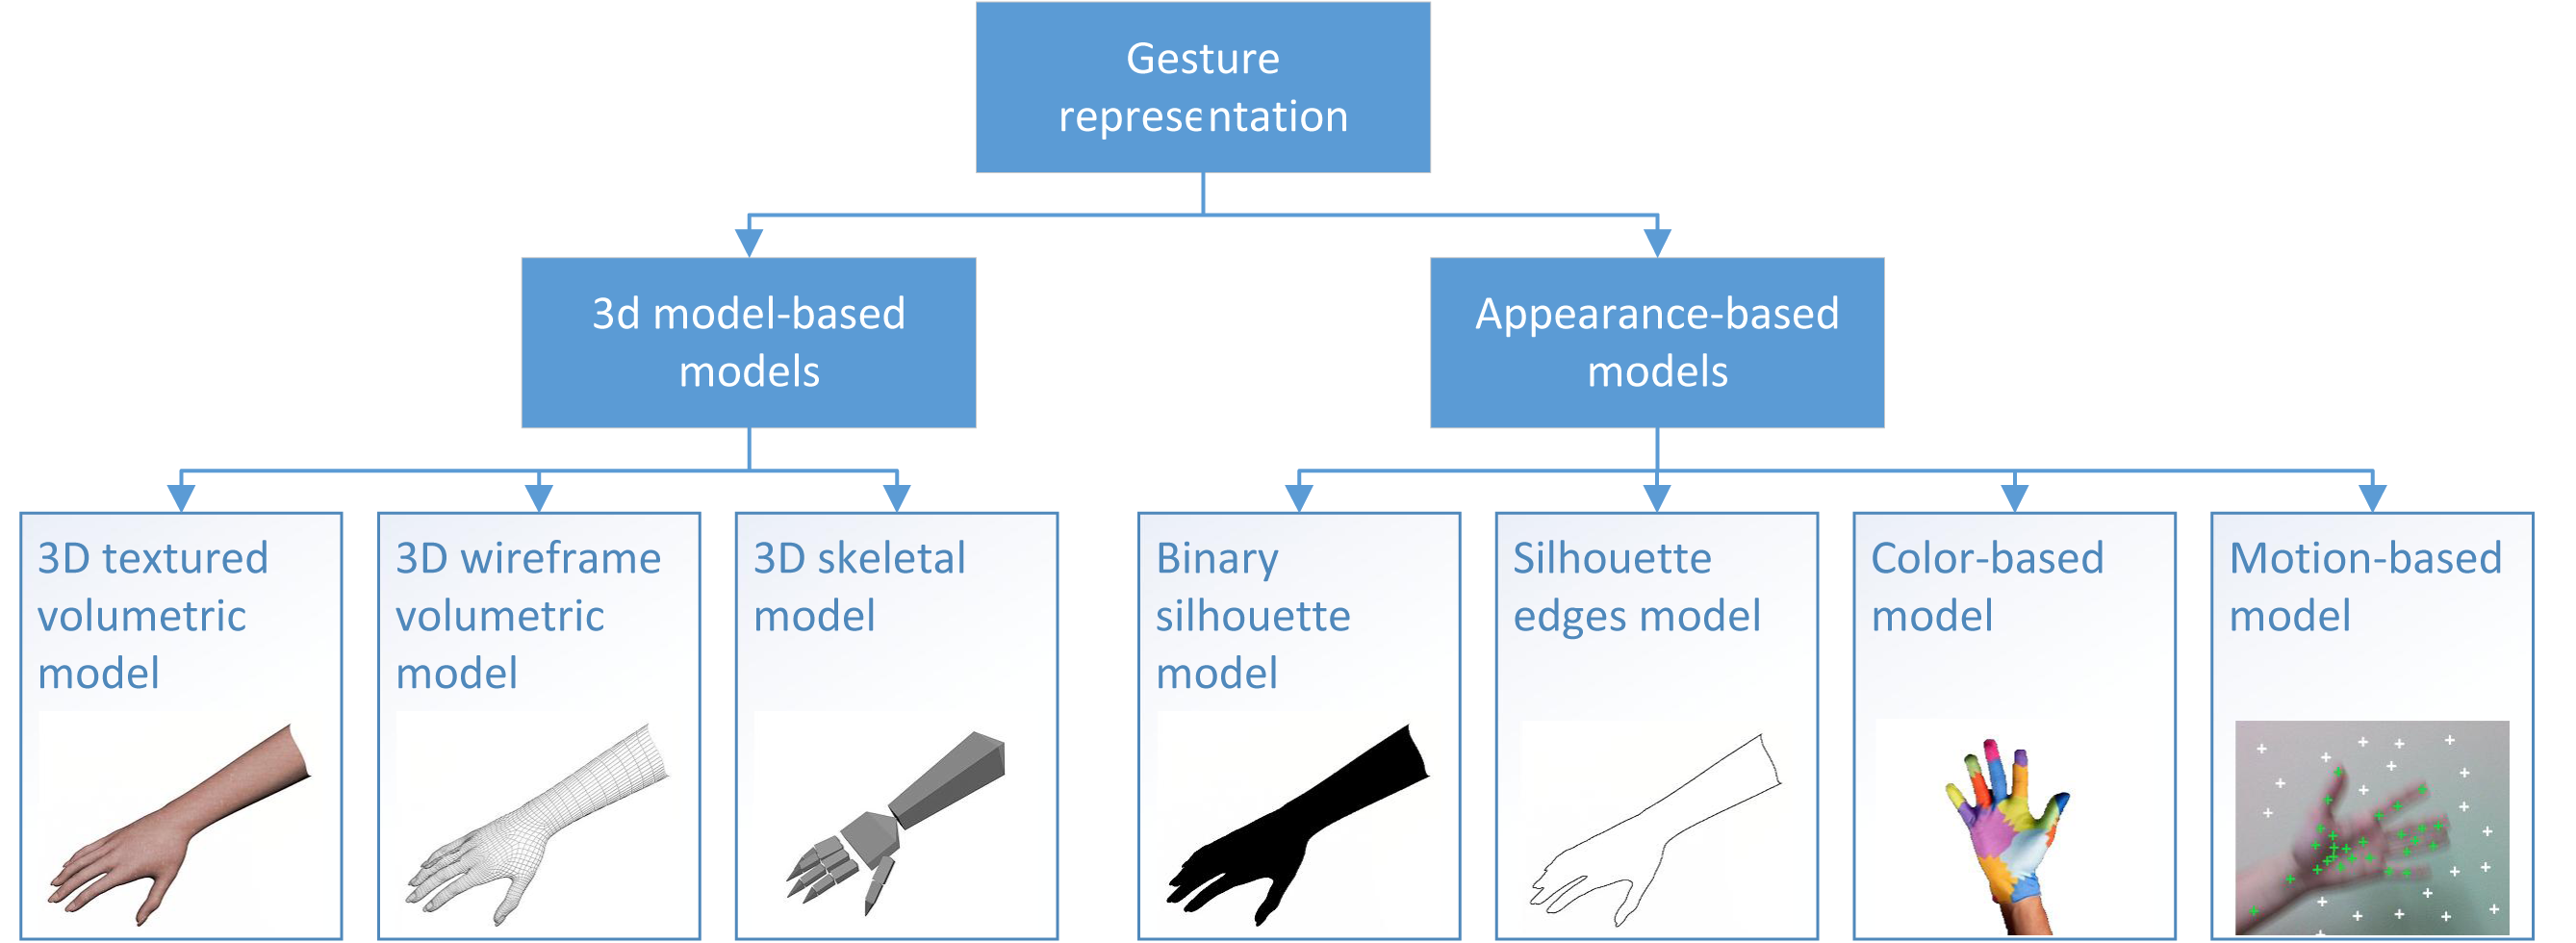
\includegraphics[width=1\columnwidth]{figures/gestureRepresentations.png}
 \caption[]{Diagram of gesture representation}
 \label{gesturerepresentations}
\end{figure}

\subsection{Gesture representation}
In this subsection, provides overview the spatial modeling of gestures. In particular, it was focused on one type of spatial gesture representations namely 3d model-based.
Depending on the type of the input data, the approach for recognize gesture could be done in different ways.
There are following two main types of gesture representation defined in literature \cite{Huang95handgesture}\cite{Pavlovic97visualinterpretation}:
\begin{itemize}
\item 3d model-based
\item Appearance-based
\end{itemize}

\subsubsection{3d model-based}

Defines the 3D spatial decription of the human body parts. They can be classified in two large groups:
\begin{itemize}
\item volumetric models
\item skeletal models
\end{itemize}
Volumetric models reproduce with high accuracy the shape of the hand or arm. Real object is often interpreted as ordered in space mesh of vertices or NURBS. This model is commonly used for computer vision purposes or to computer animation. The drawback of this approach is that is very demanding computationally and difficult to analyze in real time. With the power of today’s computers, simplified models of the hand or arm (such as skeletal models) are more recommended.

As indicated earlier, instead of dealing with all the parameters of volumetric models, model can be reduced to set of equivalent joint angle parameters together with segment lengths. Such models are known as skeletal models. There are several advantages of using skeletal models:
\begin{itemize}
\item Using simplified model with the most important parameters allows the detection program to focus on the significant parts of the body,
\item Due to the smaller amount of data, processing algorithms are faster
\end{itemize}

\subsubsection{Appearance-based}

The second group of models don’t use direct description of the spatial object points, because this model is based on shape of hands or arms in the visual images. The gestures are modeled by relating the appearance of any gesture to the appearance of the set of predefined, template gestures \cite{Pavlovic97visualinterpretation}. In this group distinguished a large variety of models. The most used 2d models are:
\begin{itemize}
\item Color based model -- in general, using body markers to track the motion of the body part,
\item Binary silhouette based model -- models based on the geometric properties of the object silhouette,
\item Deformable gabarit based model -- they are generally based on deformable active contours
\item Motion-based model -- based on the motion of individual pixels or image part description
\end{itemize}

\subsection{Gesture recognition methods}
As was written earlier, one of the main issues of gesture recognition is decision problem. Currently several solutions has been proposed, which can be used regardless of device type or data representation for different classes of gestures. Classification of gestures, which should be taken into account while choosing gesture recognition method was being chosen is static and dynamic division. For each of them may be used different tools due to the different properties of these gestures. In the case of static gesture recognition, an important feature is arrangement of object, which performs gesture. In other words how the individual parts of the object are arranged in relation to each other. For dynamic gestures -- as described in the previous subsection -- a very important feature is the variation in time (dynamics of the gesture or dynamics of individual parts of the object performing the gesture).

To recognize static gestures, general classifier, neural network or template-matcher can be used. Methods which are capable to recognize dynamic gestures have to take into account an aspect of time. The example of this kind of method is Hidden Markov Model.

\subsubsection{Static gesture recognition}

Different techniques to perform accurate static gesture recognition have been decribed in the literature. The most common methods are neural networks, support vector machines and simple pattern techniques \cite{journals/jbcs/SavarisW10}.

\emph{An neural network (NN)} is an information-processing system that has been developed as generalizations of mathematical models of human cognition or neural biology. A neural network is characterized by its pattern of connections between the neurons, method of determining the weights on the connections, and its activation function \cite{Fausett:1994:FNN:197023}. They can be used both for static and dynamic gestures.

Hasan et al. \cite{HasanStaticHand} presented hand gesture recognition based on shape analysis. Tests were conducted for six static gestures using multi-layer perception of neural network and back-propagation learning algorithm. NN architecture consisted of one hidden layer (100 nodes), 1060 inputs and 6 output for each gesture. They achieved a recognition rate of 86.38\% for a training set of 30 images and a testing set of 84 images.

Xu et al. \cite{conf/icat/XuYZ06} developed virtual training system of Self-Propelled Gun based on static gesture recognition and hand translations and rotations. The input data for algorithms was captured using a 18-sensor DataGlove. To recognize gestures was used feed-forward neural network with 40 nodes in single hidden layer, 18 input and 15 output nodes. The back-propagation using a variable learning rate is selected as training method. The tests were conducted on a set of 300 hand gestures from five different people -- 200 gestures for training set and 100 for testing set. With the use of these methods the authors reached gesture recognition performance of 98\%.

In publication of Stergiopoulou and Papamarkos publication \cite {Stergiopoulou:2009:HGR:1651923.1651954} can be found static gesture recognition through other type of neural network -- Self-Growing and Self-Organized Neural Gas (SGONG). To quote the authors, SGONG is innovative neural network that grows according to the morphology of hands in a very robust way. The algorithms were tested for 31 hand gestures that derive from the combination of shown and hidden fingers. Data were collected from a camera, and the recordings of hand were created in a vertical position on uniform background. With these assumptions, gesture recognition rate of 90.45\% have been reached but required average computation time was about 1.5 s, using a 3 GHz CPU.

\emph{Support-Vector Machine (SVM)} is a classification method invented by Vapnik \cite{Cortes:SVM}. SVM is a supervised learning algorithm used for classification and regression analysis, based on the mapping of characteristics extracted from instances namely the feature vectors to points in space. SVM constructs in multi-dimensional space, set of hyperplanes, which non-linearly divide points in this space (input vectors) to different classes. Support Vector Machines can be called a maximum margin classifier, because the resulting hyperplanes maximize the distance between the ’nearest’ vectors of different classes. These ``nearest'' vectors are called support vectors.

Chen and Tseng \cite{ChenDeveloping} presented system based on training SVM which allows effective recognition gesture in popular game, rock-paper-scissors. One of the challenges of their work was to teach the classifier to recognize multiple-angle hand gesture. The collection of training and testing data were images from video camera, which are preprocessed using convertion to grayscale and histogram equalization. Data were collected from 5 different people for the right hand only. For the learning set consisted of 420 images and testing set of 120 images, the recognition rate of 95\% was achieved.

Rahman and Afrin \cite{RahmanHand} presented hand gesture recognition system which recognizes static hand gesture for alphabet of 10 letters using Biorthogonal Wavelet Transform and SVM. Input data in the form of images -- in addition to filtering -- are transformed by the Canny edge detection method and then processed sequentially through Radon and Biorthogonal Wavelet Transformations. Finally, the data in this form are transmitted to the SVM classifier. To achieve robustness of the method to varying conditions, authors used a large dataset -- 800 positive samples and 1500 negative image samples. Average recognition rate was 87.4\%.

Liu et al. \cite{LiuStatic} proposed recognition method based on SVM and Hu moments which applied to Chinese Driver Physical Examination System. For collection of 2416 positive samples and 3050 negative samples from 20 people recognition rate of 96.5\% have been reached.

Ren and Zhang \cite{RenMEBSVM} proposed other recognition method named by them as MEB-SVM. This method combines the SVM with minimum enclosing ball (MEB) and -- according to the authors -- allows to reduce computation with effective separation of all kinds of vectors in hyperspace. The input data used to test this method are images which are initially binarized and then countour line is retrieved. Finally, contour line is converted by means of Fourier transform, so that data are independent of translation, rotating and zooming. Their method achieved a recognition rate of 92.9\%.


Dominio et al. \cite{Dominio:2013:HGR:2510650.2510651} presented novel hand gesture recognition based on depth data using Kinect device. The proposed processing consists following, main steps: extraction hand region from the depth map and subdivided it into palm and finger samples, extraction set of features based on finger tips and center of the hand, classification by SVM. Based on 1,000 different depth maps with 10 gestures performed by 10 different people, they achieved mean recognition rate of 99.5\%.

Other popular methods are \emph{simple pattern recognition techniques}. This group includes methods based on a simple comparison the characteristics of new problem instance with instances seen in training, instead of performing explicit generalization. In the case of gesture recognition, output information of algorithm is evaluated on the basis of similarity of the gesture to other pre-defined or learned gestures, for which belonging to groups is known. Basis on this, it is concluded that the newly read gesture belongs to the group. These techniques are generally based on a efficient lazy learning methods such as instance-based learning methods.  In the context of gesture recognition, the most widely used algorithm is the k-nearest neighbour.
